\let\negmedspace\undefined
\let\negthickspace\undefined
\documentclass[journal,12pt,twocolumn]{IEEEtran}
\usepackage{cite}
\usepackage{amsmath,amssymb,amsfonts,amsthm}
\usepackage{algorithmic}
\usepackage{graphicx}
\usepackage{textcomp}
\usepackage{xcolor}
\usepackage{txfonts}
\usepackage{listings}
\usepackage{enumitem}
\usepackage{mathtools}
\usepackage{gensymb}
\usepackage[breaklinks=true]{hyperref}
\usepackage{tkz-euclide} % loads  TikZ and tkz-base
\usepackage{listings}
\usepackage{gvv}
\usepackage{amsmath}

        

\newtheorem{theorem}{Theorem}[section]
\newtheorem{problem}{Problem}
\newtheorem{proposition}{Proposition}[section]
\newtheorem{lemma}{Lemma}[section]
\newtheorem{corollary}[theorem]{Corollary}
\newtheorem{example}{Example}[section]
\newtheorem{definition}[problem]{Definition}
\newcommand{\BEQA}{\begin{eqnarray}}
\newcommand{\EEQA}{\end{eqnarray}}
\newcommand{\define}{\stackrel{\triangle}{=}}
\theoremstyle{remark}
\newtheorem{rem}{Remark}

%\bibliographystyle{ieeetr}
\begin{document}
%

\bibliographystyle{IEEEtran}


\vspace{3cm}

\title{
%	\logo{
Assignment-2

\large{EE1205 : Signals and Systems}

Indian Institute of Technology Hyderabad
%	}
}
\author{Chirag Garg

(EE23BTECH11206)
}	





\maketitle

\newpage



\bigskip

\renewcommand{\thefigure}{\arabic{figure}}
\renewcommand{\thetable}{\arabic{table}}


\section{Question 11.9.1 (5)}
\vspace{0.5cm}
\begin{flushleft}
 Write the first five terms of the sequence whose $n^{th}$ \text{term is} : $x(n) = (-1)^{n-1}5^{n+1}$.
\end{flushleft} 


\vspace{0.8cm}


\section{Solution} 



\begin{table}[htbp]
\centering
\resizebox{\columnwidth}{!}{
\begin{tabular}{|c|c|c|}
    \hline
     \textbf{Parameter} & \textbf{Value} &
     \textbf{Description}\\
    \hline 
     $x(n)$ &  $(-1)^{n-1}5^{n+1}$ & General Term\\
    \hline 
     $x(0)$ &  $-5$ & First term of G.P.\\
     
    \hline
     $r$ & $-5$ & Common ratio of G.P.  \\
      \hline
    
  
								      
\end{tabular}
}
\caption{ Given Parameters}

\end{table}


On substituting n = 0, 1, 2, 3 and 4, we get the first five terms 

Hence, the required terms are -5, 25, –125, 625, –3125 .


The Z-transform of a sequence $x(n)$ is given by:

 \begin{align}
	     x(n) &= (-1)^{n-1}5^{n+1}u(n)
	       \\  X(Z) &= \dfrac{-5z}{z+5}; ( |z| > 5 )
 \end{align}


\begin{figure}
  \centering
  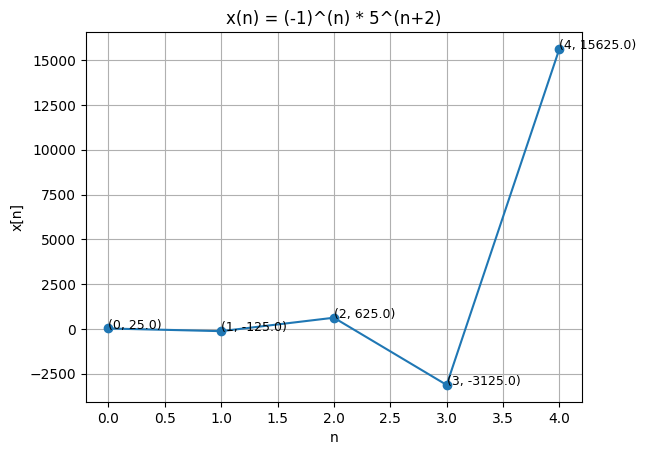
\includegraphics[width=0.5\textwidth]{figures/grasi2.png} 
 
\end{figure}


\end{document}